\let\negmedspace\undefined
\let\negthickspace\undefined
\documentclass[journal,12pt,twocolumn]{IEEEtran}
\usepackage{cite}
\usepackage{amsmath,amssymb,amsfonts,amsthm}
\usepackage{algorithmic}
\usepackage{graphicx}
\usepackage{textcomp}
\usepackage{xcolor}
\usepackage{txfonts}
\usepackage{listings}
\usepackage{enumitem}
\usepackage{mathtools}
\usepackage{gensymb}
\usepackage{comment}
\usepackage[breaklinks=true]{hyperref}
\usepackage{tkz-euclide} 
\usepackage{listings}
\usepackage{gvv}                                        
\def\inputGnumericTable{}                                 
\usepackage[latin1]{inputenc}                                
\usepackage{color}                                            
\usepackage{array}                                            
\usepackage{longtable}                                       
\usepackage{calc}                                             
\usepackage{multirow}                                         
\usepackage{hhline}                                           
\usepackage{ifthen}                                           
\usepackage{lscape}

\newtheorem{theorem}{Theorem}[section]
\newtheorem{problem}{Problem}
\newtheorem{proposition}{Proposition}[section]
\newtheorem{lemma}{Lemma}[section]
\newtheorem{corollary}[theorem]{Corollary}
\newtheorem{example}{Example}[section]
\newtheorem{definition}[problem]{Definition}
\newcommand{\BEQA}{\begin{eqnarray}}
\newcommand{\EEQA}{\end{eqnarray}}
\newcommand{\define}{\stackrel{\triangle}{=}}
\theoremstyle{remark}
\newtheorem{rem}{Remark}
\begin{document}

\bibliographystyle{IEEEtran}
\vspace{3cm}

\title{Probability Assignment}
\author{EE22BTECH11022-G.SAI HARSHITH$^{*}$% <-this % stops a space
}
\maketitle
\newpage
\bigskip
\renewcommand{\thefigure}{\theenumi}
\renewcommand{\thetable}{\theenumi}

Question: The frequency response $H(f)$ of of a linear time-invariant syatem has magnitude as shown in \figref{fig:11}\\
Statement 1: The system is necessarily a pure delay system for inputs which are bandlimited to $-a \leq f \leq a$.\\
Statement 2: For any wide-sense stationary input process with power spectral density $S_X(f)$, the output power spectral density $S_Y(f)$ obeys $S_X(f)=S_Y(f)$ for $-a \leq f \leq a$.\\
\begin{figure}[!ht]
\centering
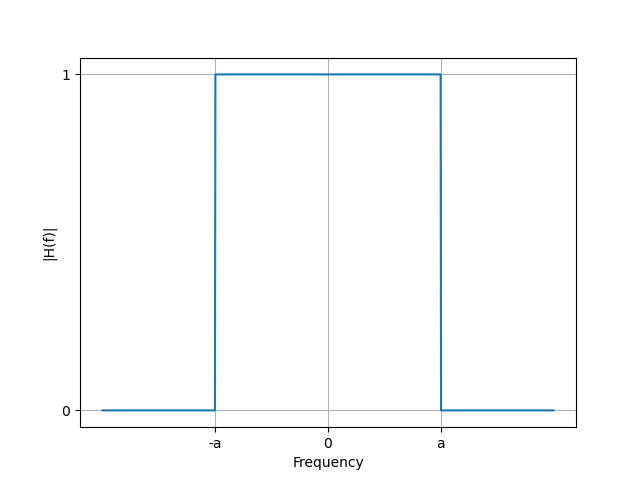
\includegraphics[width=\columnwidth]{figs/figure.png}
\caption{$|H(f)|$ vs frequency}
\label{fig:11}
\end{figure}\\
\solution
\begin{enumerate}
\item Let us consider a delay LTI system with x(t) and y(t) as input and output signals in time domian. Let $T_d$ be delay between input and output. So,
\begin{align}
y(t)&=x(t-T_d)
\end{align}
Appling fourier transform,
\begin{align}
\int_{-\infty}^{\infty}y(t)e^{-2\pi fjwt}dt&=\int_{-\infty}^{\infty}x(t-T_d)e^{-2\pi fjt}dt\\
&=\int_{-\infty}^{\infty}x(t)e^{-2\pi fj(t+T_d)}d(t+T_d)\\
&=e^{-2\pi fjT_d}\int_{-\infty}^{\infty}x(t)e^{-2\pi fjt}dt\\
Y(f)&=e^{-2\pi fjT_d}X(f)
\end{align}
Here $Y(f)$ and $X(f)$ are output and input signals in frequency domian. Let $H(f)$ be 
\begin{align}
|H(f)|&=\left|\frac{Y(f)}{X(f)}\right|\\
&=\left|e^{-2\pi fjT_d}\right|\\
&=1
\label{eq:1}
\end{align}
Here, $|H(f)|=1$ for all frequencies. But statement was for bandlimited input in $-a\leq f \leq a$. That is there is no input otherwise.  So,
\begin{align}
|H(f)| &= 
        \begin{cases}
            1 & \text{if }-a \leq k \leq a\\
            0 & \text{otherwise}
        \end{cases}\label{eq:2}
\end{align}
From \eqref{eq:2} and \figref{fig:11}, $|H(f)|$ is same.So, system will act as pure delay system. Statement 1 is correct.
\item For wide-sense stationary LTI sytem,
\begin{align}
S_Y(f)&=|H(f)|^2S_X(f)
\end{align}
Fron \eqref{eq:2}, for $-a \leq k \leq a$, $|H(f)|=1$
\begin{align}
S_Y(f)&=(1)^2S_X(f)\\
S_Y(f)&=S_X(f)
\end{align}
STatement 2 is correct.
\end{enumerate}
\end{document}
